%~~~~~~~~ Chapter ~~~~~~~~
\chapter{Quantum computing}
% this is a sentence $2\e{-3}$ or $2\cdot10^{-3}$ or $2\ex{-3}$ or $2\times10^{-3}$ with different formats and this is my state up: $\ket{\up}$\\
%
% $$2\e{-3}$$
% $$2\cdot10^{-3}$$
% $$2\ex{-3}$$
% $$2\times10^{-3}$$
%
%
% DiVincenzo's criteria for quantum computer\cite{DiVincenzo2000}:
% \begin{enumerate}
%   \item A scalable physical system with well characterized qubits.
%   \item The ability to initialize the state of the qubits to a simple fiducial state, such as $\bra{000\dots}$.
%   \item Long relevant decoherence times, much longer than the gate operation time.
%   \item A ``universal'' set of quantum gates.
%   \item A qubit-specific measurement capability.
%   \item The ability to interconvert stationary and flying qubits.
%   \item The ability to faithfully transmit plying qubits between specified locations.
% \end{enumerate}

There are moments that define history beyond our life. The Industrial revolution marked the starting point of a race that we are running even today. The automation processes that the (steam) engine started changed not only the working conditions of the world population but also the socio-economic structure of societies and even the relation of humanity with the natural world. % XXX cite global warming
The leap in the possibilities that the engine brought was bigger that anyone at the time could have predicted.

When the first computers were develop, they were able to just perform basic algebraic operations and make hard copies of the results. %XXX cite Charles Babbage and Ada Lovelace
The original purpose of computers was just to facilitate calculations, maybe fast and accurate enough to land a man in the moon, but not even the craziest dreams of the first computer engineers and programmers could grasp the impact that computers have had in the world (so far), from the creation of a worldwide repository of knowledge\cite{Stallman2000} to the hatch of revolutions through social networks\cite{Alhindi2012}. Ever since their spread in the common households computers have changed the way we interact with other people, travel, buy, even the way we vote and fight wars.
Computers have shaped societies and human relations alike and most likely they will continue doing so in the near future.

We find ourselves in a moment in which the revolution of the \acl{qc} is brewing and, quite probably, we lack the capability to capture its full potential. Nevertheless, from our limited perspective we can already see many fields were the impact of \acl{qc} will be huge.
When efficient and reliable \acp{qc} are available, a new realm of possibilities in Chemistry and Biochemistry will open, allowing the custom discovery design of complex molecules and drugs and when we master the biochemistry of living organisms there is no tell in the limit of the possibilities.
Cryptography will be forever changed once scalable, efficient \acl{qc} is commonly available. While cryptography may not be a popular discipline, it plays a major role in today's world, the secure communication over the internet. Transmission of content, personal/secret information, governmental or military information, financial transactions, all of them depend upon algorithms which will not hold under \acl{qc} calculations\cite{Shor1994}.
At the same time that \ac{qc} will tear apart our current cryptographic systems it may also hold the key for ``truly'' secure communications as quantum cryptography ensures the integrity of the information to the privacy of the same.
Even classical computers may benefit from quantum computers as algorithms for faster search and optimization have been already proposed. As the corpus of available data increases exponentially the need for an efficient algorithm to search through it\cite{Grover1997} becomes apparent. Solving optimization problems\cite{Durr2006,Montanaro2016,Brandao2017} is also an important advance that will affect many different areas, particularly \emph{Machine Learning} is one of the broad applications where these algorithms can make a difference.\footnote{Even though so far only algorithms with polynomial speed-up have been proposed for this kind of problems, it is enough to make feasible complex models for image or sound recognition, natural language processing or many other applications}\\


%XXX  nexo
The first ideas about \acl{qc} reach as far back as the 80's\cite{Benioff1980,Feynman1982}, when classical computers started their race towards miniaturization.

The ever shrinking size of the transistors\cite{Moore1965} started to point towards a possible problem as they would reach sizes in which the quantum effects could not be neglected in a few years.
Instead of focusing on the ``problem'' that the quantum effects could arise, some researchers\cite{Benioff1980,Feynman1982} considered them as an opportunity since some of these quantum effects could be exploited in our favor.

In fact, superposition, entanglement and %TODO finish
Even without any experimental (physical) playground the ideas of quantum computation started to tickle the curiosity of many scientists over the years and it became a line of research on its own. % citations!

In 2000 DiVincenzo gave a summary list of criteria for having a Quantum Computer\cite{DiVincenzo2000}, namely:
\begin{enumerate}
  \item A scalable physical system with well characterized \textbf{Qubits}. A broader discussion about what constitutes a qubit is done later so for now it suffices to say that a qubit is a quantum two-level system. For instance the two spin states of a $\tfrac{1}{2}$ particle in a Zeeman magnetic field, or the vertical/horizontal polarization of a single photon.
  \item The ability to reliably \textbf{initialize} the state of the qubits to a simple state, such as $\bra{000\dots}$. There are two main reasons for this requirement. The first one is that registers should be initialized to some known value before the beginning of the computation. The second one is that quantum error operations require a continuous, fresh supply of qubits in a low-entropy state. The rate at which the qubits can be zeroed will set an important time scale for many other operations.
  \item \textbf{Long} relevant \textbf{decoherence times}. The actual requirement is not that the decoherence time is long, but that it is much longer than the gate operation time.
  \item A ``universal'' set of \textbf{quantum gates}.\cite{Deutsch1985,Deutsch1989} \acl{qc}, as classical, require logical gates to perform operations. Classical gates, such as OR,XOR,AND,NAND,... have a quantum version. Quantum gates work by rotating the qubit states in the Bloch space (see Fig.~\ref{Bsph}) what can result in states that do not exist in classical bits, hence, there are some quantum gates without a classical counterpart. There are gates that act in one qubit and gates that require two (or more) qubits to operate. Regardless of the embodiment of the qubits the logic gates are required to be as fast as possible since the duration of the operations will set the time scale for the decoherence time.
  \item A qubit-specific \textbf{measurement} capability. Depending on the physical implementation the measurement procedure will vary, but in any case some properties are always desirable. For instance, if the qubit's density matrix is $
    \rho = p\ket{\up}\bra{\up} + (1-p)\ket{\down}\bra{\down} +
           \alpha\ket{\down}\bra{\up} + \alpha^\dagger\ket{\up}\bra{\down}
  $ the measurement should result in $\up$ with probability $p$ and in $\down$ with probability $(1-p)$ regardless of the parameter $\alpha$ (or any other parameter, for that matter). Also, it would be desirable that the measurement process of one specific qubit does not affect any of the other qubits. If these requirements are not completely met, then the efficiency is said to be smaller than $100\%$ , which does not mean that is not enough to work. As a rule of thumb, for a quantum computer to work with an efficiency $q$, more than $1/q$ are required, so the result is robust enough.
\end{enumerate}
optionally, for other tasks, mainly communication related (such as secret key distribution or multiparty function evaluation)\cite{DiVincenzo1999}, two more features would be desirable:
\begin{enumerate}
  \setcounter{enumi}{6}
  \item The ability to interconvert stationary and flying qubits\cite{Turchette1995,Imamoglu1999}.
  \item The ability to faithfully transmit flying qubits between specified locations.
\end{enumerate}
%TODO understand these 2


We are going to delve  now in the definition





\section{What is a Qubit?}
In classical computing the basic element of information is a known as a bit. All the information that we can think of in our computers is encoded in a set of bits.
For instance one of the most famous ways of encoding text is the so-called \ac{ascii} encoding, in this case we use 7 bits to encode all the letters and numbers and some symbols, for instance $a=\texttt{1100001}$, $A=\texttt{10000011}$, $b=\texttt{1100010}$, and so on.

Classical bits can only take two values, namely \texttt{0} or \texttt{1}, $+$ or $-$, $\uaw$ or $\daw$, and all the operations that we do in our everyday lives is restricted to flip or not the states of some bits, from photograph editing, to music players, to web browsing, to the hardest scientific calculations, everything that requires a computer at the end of the day is just flipping the correct bits.

% Current processors operate on 64bits each time, taking into account that an standard computer operates at $\approx 2\cdot10^9 MHz$ it means that this can operate about $100\cdot10^9$ bits per second

There are many different types of bits. In early computers a bit would be a hole in a cardboard and its states would be the presence or absence of a hole. Later on it would be electrically controlled like an electrical switch, or a flip-flop circuit, or any other system with two different states that can be easily manipulated.

Recent computers use the magnetization of small cells as bits. This means that the physical representation of a bit of classical information nowadays is just a bunch of spins pointing in one direction or the other.
Even when spins are intrinsically quantum objects in current computers no intrinsically quantum property is exploited.
In the last 30 or 40 years there has been a continuous effort to reduce the size of the bits in order to get a higher density of information in our devices. This trend lead people to consider what would happen when the bits become small enough for the quantum effects to be relevant. And here is where the idea of Quantum bits appeared.
The qubit.

% Of course, the consequences of considering \acp{qb} go far beyond the miniaturization of memories and devices.

The simplest possible representation of a \ac{qb} is a \ac{2ls}. A system with two well defined (and physically distinguishable) states. The Hilbert state of such a system will consist of a basis of two independent states, namely $\mathcal{B}=\{\ket{\up},\ket{\down}\}$. We will use this notation independently of the physical realization of the \ac{qb}, whether they are spin $\tfrac{1}{2}$ systems, polarization of photons, or discrete level in a confined system.
As opposed to classical bits, a \ac{qb} in general will be in a combination of the states of the basis:
\begin{equation}
  \ket{\psi} = \alpha\ket{\up} + \beta\ket{\down} \qquad\text{with}\qquad
  |\alpha|^2+|\beta|^2 =1
               % \cos\frac{\theta}{2}\ket{\up} + e^{i\phi}\sin\frac{\theta}{2}\ket{\down} =
\label{genstate}
\end{equation}
% If the chosen physical representation for the \ac{qb} would be a spin $S=1/2$ in the presence of a magnetic field, the geometrical interpretation of such an state shown in figure~\ref{Bsph}. Nevertheless many physical implementations of qubits exist nowadays, so the interpretation of the general state is not universal.
%~~~~~~~~~~~~~~~~~~~~~~~~~~ FIGURE ~~~~~~~~~~~~~~~~~~~~~~~~~%
\begin{figure}[!h]
\centering
% 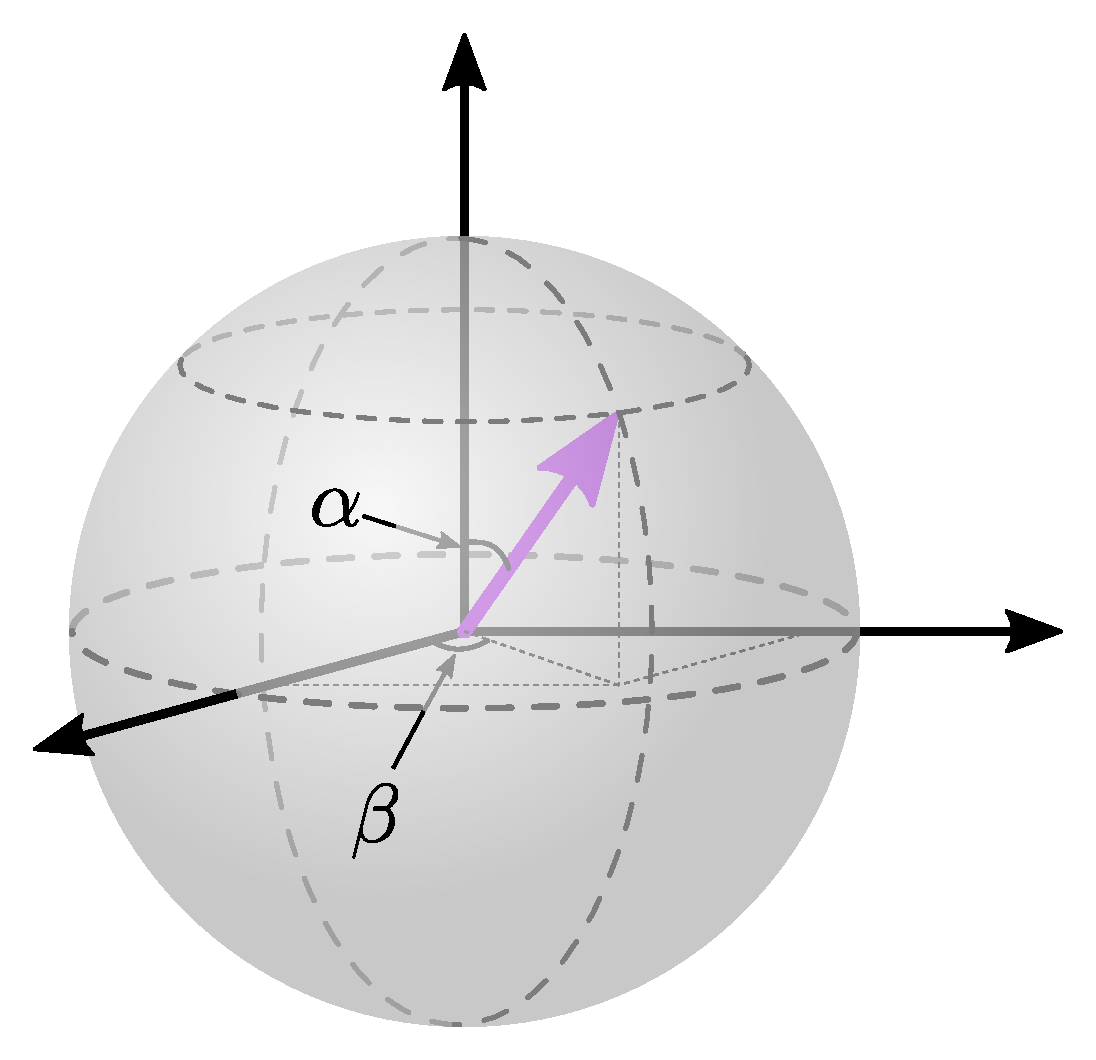
\includegraphics[width=0.5\textwidth]{chapter01/figures/bloch_sphere.png}
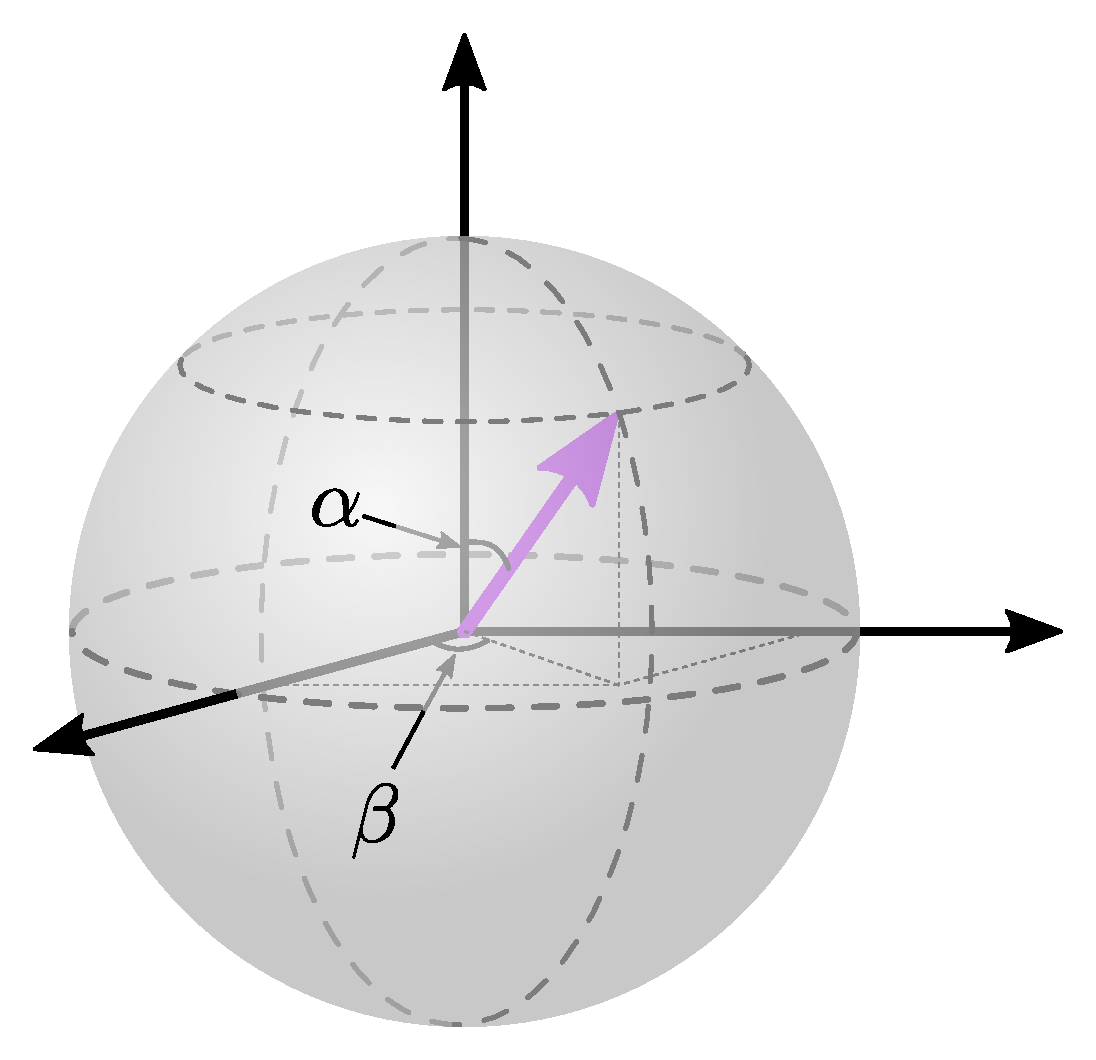
\includegraphics{chapter01/figures/bloch_sphere.pdf}
\vspace{-5pt}
\caption{Bloch sphere that represents all the possible states of a qubit.}
\label{Bsph}
\end{figure}
\FloatBarrier
%~~~~~~~~~~~~~~~~~~~~~~~~~~~~~~~~~~~~~~~~~~~~~~~~~~~~~~~~~~~%
Notice that as opposed to classical bits, a single \ac{qb} can exist in a continuum of states which can be mapped to any 2D space, usually that space is chosen to be the surface of a sphere such as that shown in Fig.~\ref{Bsph}, commonly known as Bloch sphere.

Nevertheless the idea of having qubits goes far beyond the possibility of storing more states per qubit (in fact probably quantum memories will not be such a great idea since they could be quite volatile).
The great advantage that the \ac{qc} brings is that we can actually perform operations not only in each of the basis states but in combinations of these states\cite{DiVincenzo2000}. In the case of a single qubit, the space in which any state can be expanded is ``only'' 2D, but if we consider three \ac{qb} the general state would be
\begin{equation}
  \ket{\psi} = \alpha\ket{\up;\up} + \beta\ket{\up;\down} +
               \gamma\ket{\down;\up} + \delta\ket{\down;\down}
\end{equation}
which lives in a 4D space (2n).
If a ``complete'' quantum computer were build, the space of state that it could access would be a $2^n$ space, with $n$ the number of qubits in the system. Being able to perform operations on such a complex states would allow an effective massive parallelization on a scale far beyond any technological expectation.
In fact it is not just a matter of scale. The possibility of accessing such complexity opens a whole new realm of problems that we can approach.

The basic cryptographic principles used nowadays to protect on-line communications relay on our current impossibility of finding the prime factors of big numbers\cite{Shor1994}.
The parameter space that describes the folding of proteins is so huge that it is impossible to explore (computationally) to design custom molecules.\cite{Lanyon2009}
database searching\cite{Grover1997}
traveling salesman\cite{Goswami2004, Moylett2017}




\section{An example: the Deutsch's problem}
This problem is the simplest example where a quantum speed up is demonstrated~\cite{Deutsch1992}. Even when the speed up is only a factor $\times2$ and the problem is purely academic, it contains all the ingredients to understand the essence of quantum computing.

The Deutsch's problem can be stated as follows:

\paragraph{Given an unkown black box that works as a binary 1 bit function $f(x)$, how can we know if it is a constant function, or a balanced function evaluating it only once?\\}
\textcolor{white}{.}\\
Notice that there are only 4 possible functions (see table~\ref{binfunc}) that take one input with two possible states and returns one output with two possible states.
\begin{table}[h!]
\begin{center}
\begin{tabular}{c|c|c|c|c}
% \hline
\multicolumn{1}{l|}{Input} & \multicolumn{1}{l|}{$A$} & \multicolumn{1}{l|}{$B$} & \multicolumn{1}{l|}{$C$} & \multicolumn{1}{l}{$D$} \\ \hline
$\up$ & $\up$ & $\up$ & $\down$ & $\down$ \\ %\hline
$\down$ & $\up$ & $\down$ & $\up$ & $\down$ \\ %\hline
% 0 & 0 & 0 & 1 & 1 \\ %\hline
% 1 & 0 & 1 & 0 & 1 \\ %\hline
\end{tabular}
\end{center}
\vspace{-15pt}\caption{The only four possible binary functions of 1 bit}
\label{binfunc}
\end{table}

On one hand we have the options $A$ and $D$ that always return either 0 or 1 regardless of the input, for this reason we will refer to them as constant functions.
On the other hand, $B$ and $C$ flips or not one of the states. In fact, using classical computation language, $B$ and $C$ perform the NOT function. We will refer to these options as balanced functions.\\

Classically to solve the Deutsch's problem (find if the black-box $f(x)$ is balanced or constant) we need to evaluate the function for both inputs.

If we measure the input $\up$, and get $\up$: $f(\up)=\up$ the function could be either $A$ (constant) or $B$ (balanced), so we need to know the behavior of $f(\down)$ to distinguish between these two possibilities.
There is no way around it. No matter how we address this problem, classically, we will always need to evaluate the function twice.

But quantum computation offers the resources to figure out the nature of the function $f(x)$ with only one evaluation. To understand how this works we just need to define two quantum gates.

The description of the gates (and the problem) will be done for a generic qubit with two states $\ket{\up}$ and $\ket{\down}$.

\subsection{Notation}
Depending on the physical implementations of the Qubits, the physical interpretation may change. Either $0/1$, $+/-$, $\uaw/\daw$ are valid We may use indistinctly the following notation
%TODO fix notation
\begin{equation}
  \ket{\up} = \ket{\uaw} =
  \left(\begin{array}{c}
        1 \\
        0
        \end{array}\right)
\qquad;\qquad
  \ket{\down} = \ket{\daw} =
  \left(\begin{array}{c}
        0 \\
        1
        \end{array}\right)
\end{equation}



\subsection{The Hadamard Gate}
The Hadamard gate acts on a single qubit by mapping the states as follows:
\begin{equation}
  \ket{\up} \longrightarrow \frac{\ket{\up}+\ket{\down}}{\sqrt{2}}
  \qquad;\qquad
  \ket{\down} \longrightarrow \frac{\ket{\up}-\ket{\down}}{\sqrt{2}}
  % \ket{0} \longrightarrow \frac{\ket{0}+\ket{1}}{\sqrt{2}} \quad\quad;\quad\quad
  % \ket{1} \longrightarrow \frac{\ket{0}-\ket{1}}{\sqrt{2}}
\label{Hmap}
\end{equation}
The matrix representation (in the basis $\mathcal{B}=\left\{\ket{\up},\ket{\down}\right\}$) is:
% The matrix representation (in the basis $\mathcal{B}=\left\{\ket{0},\ket{1}\right\}$) is:
\begin{equation}
  H=\frac{1}{\sqrt{2}}\left(\begin{array}{cc}
  1 & 1 \\
  1 & -1
  \end{array}\right)
\label{hadamard}
\end{equation}
Notices that this gate is an unitary operation: $H\cdot H^{\dagger}=\mathbb{I}$.

To understand what this gate means physically it is useful to imagine our qubit as an spin $1/2$ particle in the presence of a magnetic field.
In this physical representation the Hadamard gate would correspond to switching on a magnetic field along the $X$ direction for a certain time so the state initially in the $\pm1_z$ state would evolve to the $\pm1_x$ state.

In other physical implementation this gate would require a different physical process, but its action needs to be the mapping described in \eqref{Hmap}.


\subsection{The CNOT Gate}
The other gate that we need is the CNOT gate. This is a 2-qubit function that flips the second qubit state only if the first qubit is in the state $1$. For describing the state of the two qubits we need an slightly more complex basis:
\begin{equation}
  \mathcal{B}=\left\{
  \ket{\up;\up},\ket{\up;\down},\ket{\down;\up},\ket{\down;\down}
  \right\}
\end{equation}
\red{Modify notation} In this notation the subindex $1,2$ refers to the qubit, and the value $0,1$ refers to the state of the corresponding qubit that are chosen to be the eigenvectors of the $S_z$ operator.
In this basis the CNOT gate would be expressed:
\begin{equation}
  \text{CNOT}=\left(\begin{array}{cc|cc}
  1 & 0 & 0 & 0 \\
  0 & 1 & 0 & 0 \\\hline
  0 & 0 & 0 & 1 \\
  0 & 0 & 1 & 0
  \end{array}\right)
\end{equation}
Notice that this gates %XXX (as all the gates)
is also unitary, meaning that $\text{CNOT}\cdot\text{CNOT}^{\dagger}=\mathbb{I}$


If we think again in the spin $1/2$ particle in a magnetic field as the physical representation this function would be the process of measuring the first qubit state and applying a magnetic field in the $X$ only if the state of the first qubit is in the state $\ket{\down}$ % +1

The mapping that this function performs in our basis vectors is the following:
\begin{equation}
  \begin{split}
    &\ket{\up;\up}\rightarrow\ket{\up;\up} \qquad;\qquad
    \ket{\up;\down}\rightarrow\ket{\up;\down}\\
    &\ket{\down;\up}\rightarrow\ket{\down;\down} \qquad;\qquad
    \ket{\down;\down}\rightarrow\ket{\down;\up}
    % &\ket{0_10_2}\rightarrow\ket{0_10_2} \quad\quad;\quad\quad
    % \ket{0_11_2}\rightarrow\ket{0_11_2}\\
    % &\ket{1_10_2}\rightarrow\ket{1_11_2} \quad\quad;\quad\quad
    % \ket{1_11_2}\rightarrow\ket{1_10_2}
  \end{split}
\end{equation}
Since we are using the eigenvectors of each qubit as building blocks for our basis, all the states can be expressed as product states\blue{rephrase}. Expressing the previous mapping in these terms will be useful later on.
Any state of the basis $\ket{\phi_i}$ can be expressed as direct product of the the state of the first qubit $\ket{x}$ and the state of the second qubit $\ket{y}$, this is  $\ket{\phi_i}=\ket{x}\otimes\ket{y}$.
Using this notation, the mapping for the CNOT function can be written as follows:

\begin{equation}
  \begin{array}{lcl}
    \ket{x} & \longrightarrow & \ket{x} \\
    \ket{y} & \longrightarrow & \ket{x\oplus y}
  \end{array}
\end{equation}
this means that the CNOT gate is equivalent to apply a \ac{xOr}\footnote{The XOR gate (2 bits for the input) is a controlled NOT gate (1 bit input) that reverses the second qubit only if the control bit takes value $\down$.} controlled by the first qubit. It is useful to remember that XORding any input with 0 ($\up$) returns the same input while XORding any input with 1 ($\down$) returns the opposite input, denoted by a tilde.
\begin{equation}
  \up\oplus y = y \qquad;\qquad \down\oplus y = \tilde{y}
\end{equation}

With these two gates we are ready to address the Deutsch's problem using quantum computation.

\subsection{The Deutsch's Problem}
The formal proposal of the Deutsch's problem\footnote{the original problem deals with a function $f:\{ 0,1\}^n\rightarrow\{ 0,1\}$, but the simplest case, $n=1$, is enough to understand all the ingredients needed for quantum computation} is the following:\\

We are given a black box quantum computer known as an oracle that implements some function $f:\{ 0,1\}\rightarrow\{ 0,1\}$, this is, it takes n-digit binary values as input and produces either a 0 or a 1 as output for each such value. We are promised that the function is either constant (0 on all inputs or 1 on all inputs) or balanced (returns 1 for half of the input domain and 0 for the other half); the task then is to determine if $f$ is constant or balanced by using the oracle as few times as possible. \\

This means that there would be a quantum speed-up if we could distinguish whether
\begin{equation}
  f(\up) = f(\down) \qquad \text{or}\qquad f(\up) = \tilde{f(\down)}
  % f(0) = f(1) \quad\quad \text{or}\quad\quad f(0) = \tilde{f}(1)
  \label{problem}
\end{equation}
evaluating the function $f(x)$ only once.\\

This is in fact possible by using two qubits $x$, $y$, and some quantum gates. The complete scheme can be seen in figure~\ref{fcnot}.
%~~~~~~~~~~~~~~~~~~~~~~~~~~ FIGURE ~~~~~~~~~~~~~~~~~~~~~~~~~%
\begin{figure}[!h]
  \centering
  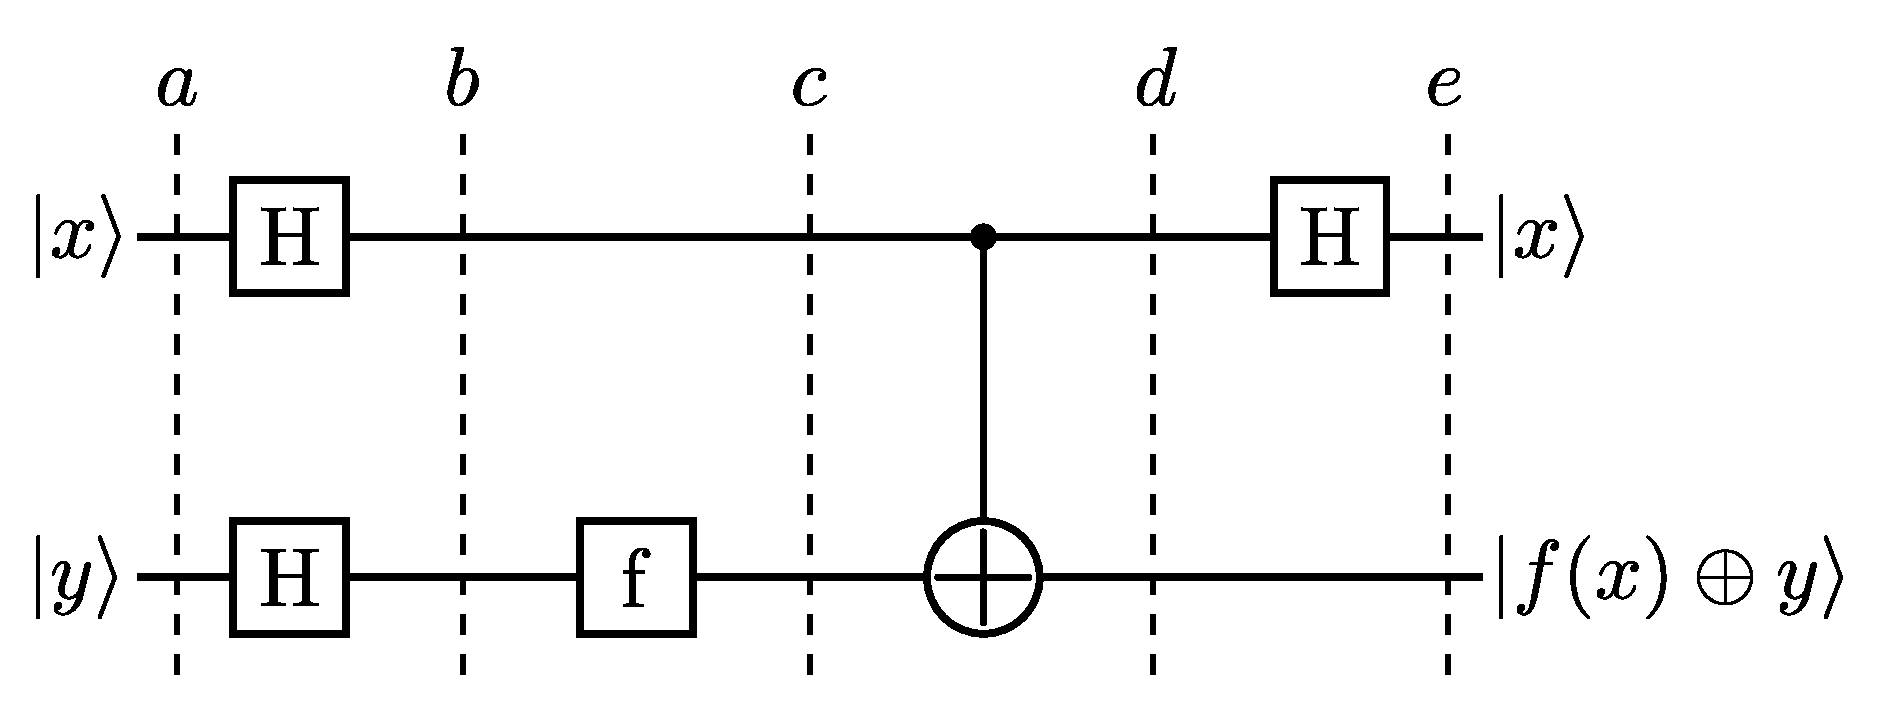
\includegraphics{chapter01/figures/fcnot.pdf}
  \vspace{-5pt}
  \caption{Scheme of the system used for solving the Deutsch's problem. The H boxes represent Hadamard gates, and the I box is am identity gate. The different stages of the algorithm are marked by letters a,b,c,d.}
  \label{fcnot}
\end{figure}
\FloatBarrier
%~~~~~~~~~~~~~~~~~~~~~~~~~~~~~~~~~~~~~~~~~~~~~~~~~~~~~~~~~~~%
As stated before, classically we would need to evaluate the oracle $f(x)$ twice, while using a quantum computer we would only need to do it once. To  do so we will use a modified CNOT gate such that one of the input bits is evaluated by the $f$ function. This can be expressed as follows
\begin{equation}
  \begin{array}{lcl}
    \ket{x} & \longrightarrow & \ket{x} \\
    \ket{y} & \longrightarrow & \ket{f(x)\oplus y}
  \end{array}
  \label{fCNOT}
\end{equation}
Notice that this modified CNOT gate (fCNOT) only evaluates the function on one of the qubits, $f(x)$.\\


In the initial state (stage $a$) we will have both qubits in the same state. We will use the following notation:
\begin{equation}
  \ket{\psi_{a}} = \ket{\up;\up} \qquad\text{or equivalently}\qquad
  \ket{x}=\up\text{, }\ket{y}=\up
  % \ket{\psi_{a}} = \ket{1_11_2} \quad\quad;\quad\quad (\ket{x}=1, \ket{y}=1)
\end{equation}
We run each qubit through a Hadamard gate, eq \eqref{hadamard}, so the state at the stage $b$ would be:
\begin{equation}
  \ket{\psi_{b}} =
  \left(\frac{\ket{\up}-\ket{\down}}{\sqrt{2}}\right)\otimes
  \left(\frac{\ket{\up}-\ket{\down}}{\sqrt{2}}\right) =
  \frac{1}{2}\left(\ket{\up;\up}-\ket{\up;\down}-
  \ket{\down;\up}+\ket{\down;\down}\right)
  % \ket{\psi_{b}} =
  %  \left(\frac{\ket{0_1}-\ket{1_1}}{\sqrt{2}}\right)\otimes
  %  \left(\frac{\ket{0_2}-\ket{1_2}}{\sqrt{2}}\right) =
  % \frac{1}{2}\left(\ket{0_10_2}-\ket{0_11_2}-
  %                  \ket{1_10_2}+\ket{1_11_2}\right)
\end{equation}
Notice that this state $\ket{\psi_b}$ is a \textbf{non-entangled superposition of all the possible inputs}, so by just one evaluation of the $f(x)$ function we would be calculating all the possible outputs simultaneously.

This is where the great advantage of the quantum computation becomes apparent since it allows the simultaneous evaluation of many different inputs as a superposition of them.

When we feed the state $\ket{\psi_b}$ to the f-CNOT gate we would get the following state at the stage $c$
\begin{equation}
  \ket{\psi_{c}} = \frac{1}{2}
  \left(\ket{\up;f(\up)} - \ket{\down;f(\down)} - \ket{\up;\tilde{f}(\up)}+
  \ket{\down;\tilde{f}(\down)} \right)
  % \ket{\psi_{c}} = \frac{1}{2}
  % \left(\ket{0_1f(0_1)_2} - \ket{1_1f(1_1)_2} - \ket{0_1\tilde{f}(0_1)_2}+
  % \ket{1_1\tilde{f}(1_1)_2} \right)
\end{equation}
In case this is not clear, let's do the explicit calculation. Using the shortcut \eqref{fCNOT}
For the first two terms:
\begin{equation}
  \begin{split}
    \text{f-CNOT}\ket{\up;\up} &=
    \ket{\up}\otimes\ket{f(\up)\oplus\up} =\ket{\up;f(\up)}\\
    \text{f-CNOT}\ket{\down;\up} &=
    \ket{\down}\otimes\ket{f(\down)\oplus \up} = \ket{\down;f(\down)}
    % \text{f-CNOT}\ket{0_10_2} &=
    %  \ket{0_1}\otimes\ket{f(0_1)\oplus 0_2} =  \ket{0_1 f(0_1)_2}\\
    % \text{f-CNOT}\ket{1_10_2} &=
    %  \ket{1_1}\otimes\ket{f(1_1)\oplus 0_2} = \ket{1_1 f(1_1)_2}
  \end{split}
\end{equation}
Notice that the evaluation of $f(x)$ is now XORded with 0 ($\up$), coming from the first qubit, so the second qubit should not be modified.
In case the notation gets messy let's point out that $\ket{\down;f(\down)}$ will be either $\ket{\down;\up}$ or $\ket{\down;\down}$, depending on the behavior of $f(x)$.

The calculation for the last two terms yields:
\begin{equation}
  \begin{split}
    \text{f-CNOT}\ket{\uaw;\daw} &=
    \ket{\uaw}\otimes\ket{f(\uaw)\oplus \daw} = \ket{\uaw;\tilde{f}(\uaw)}\\
    \text{f-CNOT}\ket{\daw;\daw} &=
    \ket{\daw}\otimes\ket{f(\daw)\oplus \daw} = \ket{\daw;\tilde{f}(\daw)}
    % \text{f-CNOT}\ket{0_11_2} &=
    %  \ket{0_1}\otimes\ket{f(0_1)\oplus 1_2} = \ket{0_1\tilde{f}(0_1)_2}\\
    % \text{f-CNOT}\ket{1_11_2} &=
    %  \ket{1_1}\otimes\ket{f(1_1)\oplus 1_2} = \ket{1_1\tilde{f}(1_1)_2}
  \end{split}
\end{equation}
Notice that the evaluation of $f(x)$ is now XORded with 1 ($\down$), hence it will be flipped.\\

Now, depending on the unknown nature of $f(x)$, eq \eqref{problem}, we could rewrite $\ket{\psi_c}$ in two different ways.
\begin{equation}
  \begin{split}
    &\text{if f is constant:   }f(\up)=f(\down)\quad\Rightarrow\quad
    \ket{\psi_c}=
    \frac{1}{2}(\ket{\up}-\ket{\down})\otimes
    (\ket{f(\up)}-\ket{\tilde{f}(\up)})\\
    &\text{if f is balanced:   } f(\up)=\tilde{f}(\down)\quad\Rightarrow\quad
    \ket{\psi_c}=
    \frac{1}{2}(\ket{\up}+\ket{\down})\otimes
    (\ket{f(\up)}-\ket{\tilde{f}(\up)}) \\
    % &\text{if f is constant:   }f(0)=f(1)\quad\Rightarrow\quad
    % \ket{\psi_c}=
    % \frac{1}{2}(\ket{0_1}-\ket{1_1})\otimes
    %            (\ket{f(0_1)_2}-\ket{\tilde{f}(0_1)_2})\\
    % &\text{if f is balanced:   } f(0)=\tilde{f}(1)\quad\Rightarrow\quad
    % \ket{\psi_c}=
    % \frac{1}{2}(\ket{0_1}+\ket{1_1})\otimes
    %            (\ket{f(0_1)_2}-\ket{\tilde{f}(0_1)_2}) \\
  \end{split}
\end{equation}


Notice that the state of the first qubit ($\up$ or $\down$) depends on whether the function $f(x)$ is constant or balanced, so just by running the state of the first qubit through a Hadamard gate we can know the nature of the function $f$:
\begin{equation}
  \begin{split}
    &\text{if f is constant:   }f(\up)=f(\down)\quad\Rightarrow\quad
    \ket{\psi_d}= \ket{\down}\otimes(\ket{f(\up)}-\ket{\tilde{f}(\up)})\\
    &\text{if f is balanced:   } f(\up)=\tilde{f}(\down)\quad\Rightarrow\quad
    \ket{\psi_d}= \ket{\up}\otimes(\ket{f(\up)}-\ket{\tilde{f}(\up)})
    % &\text{if f is constant:   }f(0)=f(1)\quad\Rightarrow\quad
    % \ket{\psi_d}= \ket{1_1}\otimes(\ket{f(0_1)_2}-\ket{\tilde{f}(0_1)_2})\\
    % &\text{if f is balanced:   } f(0)=\tilde{f}(1)\quad\Rightarrow\quad
    % \ket{\psi_d}= \ket{0_1}\otimes(\ket{f(0_1)_2}-\ket{\tilde{f}(0_1)_2})
  \end{split}
\end{equation}

If the final state of the first qubit after the whole process is $\ket{\down}$, then we know that $f(x)$ is a constant function whereas if the final state is $\ket{\up}$ we know that $f(x)$ is balanced.\\

The main point in this example is that the function $f(x)$ \textbf{was executed only once, but it was executed on a superposition state containing all the possible inputs}.\\

Naturally this is the simplest example possible, and it only provides a $\times2$ speed up in a (not really relevant) problem. Nevertheless these concepts can be applied to many other algorithms allowing a huge speed up in very important problems such as factoring big numbers, critical for current encryption systems (Shor's algorithm, that runs in polynomial time) or searching in databases, important in unsupervised machine learning algorithms (Grover's algorithm $\mathcal{O}(n)\rightarrow\mathcal{O}(\sqrt{n})$)

\red{quantum chemistry, Quantum simmulations and stuff, proteins...}.

%~~~~~~~~~~~~~~~~~~~~~~~~~~ FIGURE ~~~~~~~~~~~~~~~~~~~~~~~~~%
\begin{figure}[!h]
  \centering
  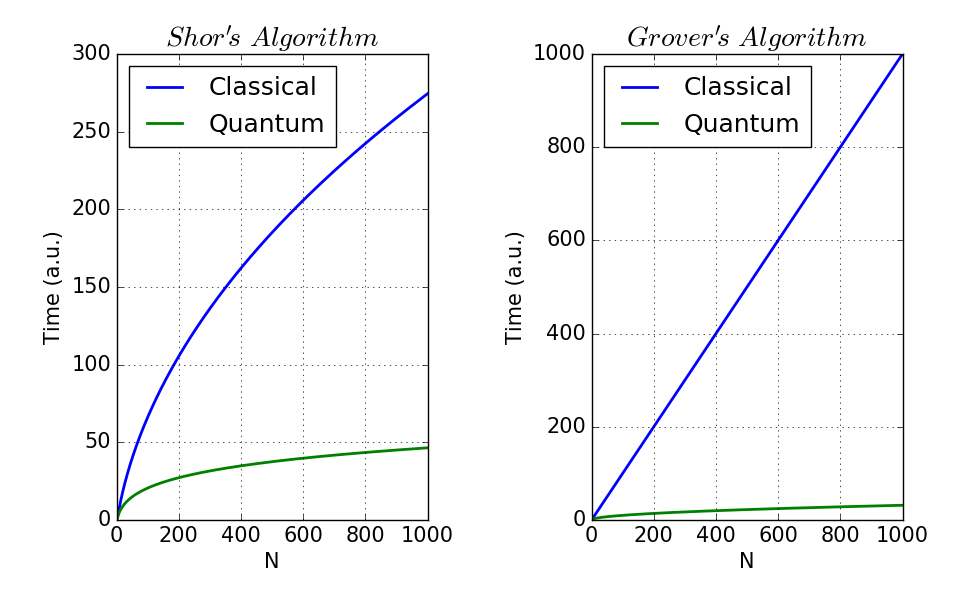
\includegraphics{chapter01/figures/quantum_scaling.png}
  \vspace{-5pt}
  \caption{Time order of the Shor and Grover's algorithm. Here we plot the scaling of the analogue classical algorithms (the best scaling we know so far) and the order of the quantum algorithm. Quantum computers allow a drastic change in the scaling of these algorithms.}
\end{figure}
\FloatBarrier
%~~~~~~~~~~~~~~~~~~~~~~~~~~~~~~~~~~~~~~~~~~~~~~~~~~~~~~~~~~~%


\section{Material realizations}
\begin{itemize}
  \item superconductor transmon
  \item majorana
  \item trapped ions
\end{itemize}
